%webservice
\subsection{Description}\label{ssec:WedDesc}

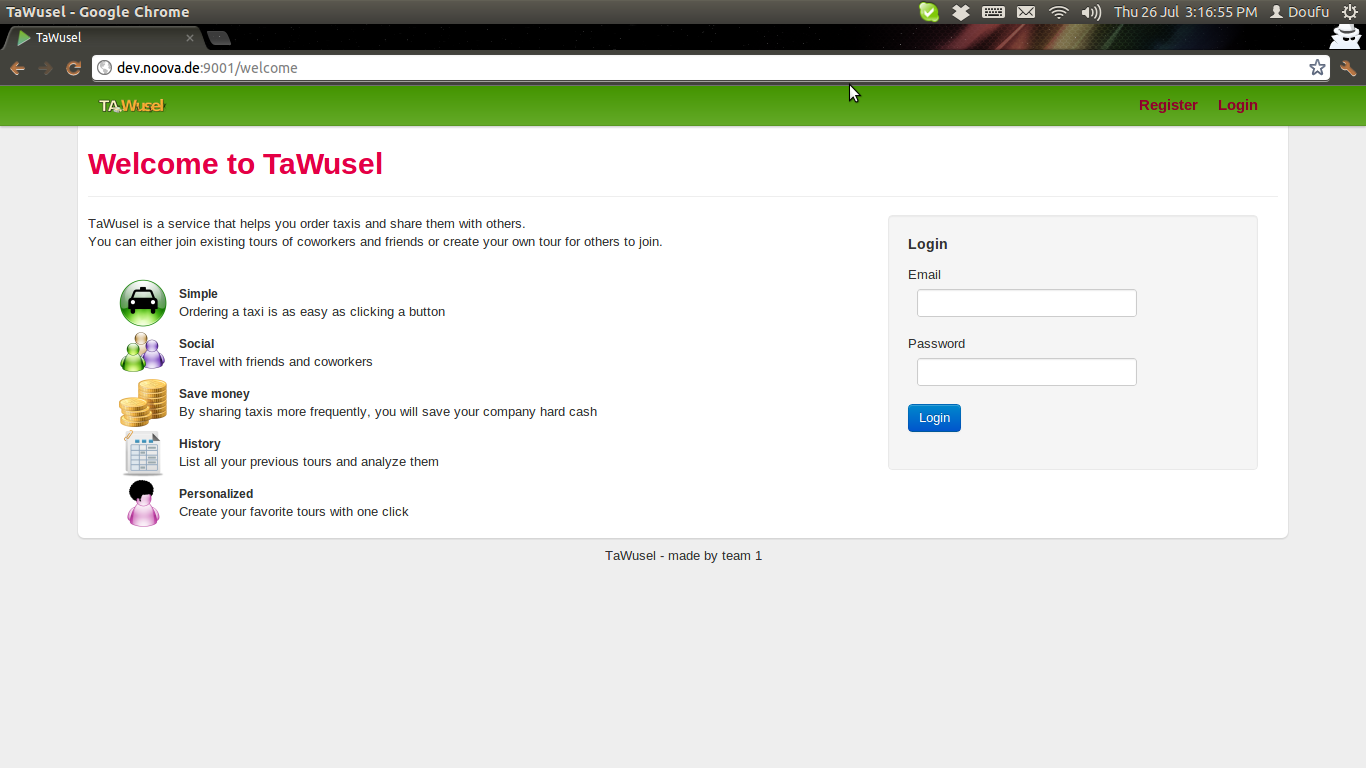
\includegraphics[width=16cm]{images/TaWusel_Web_Login.png}\label{img:WebLogin}
blabla


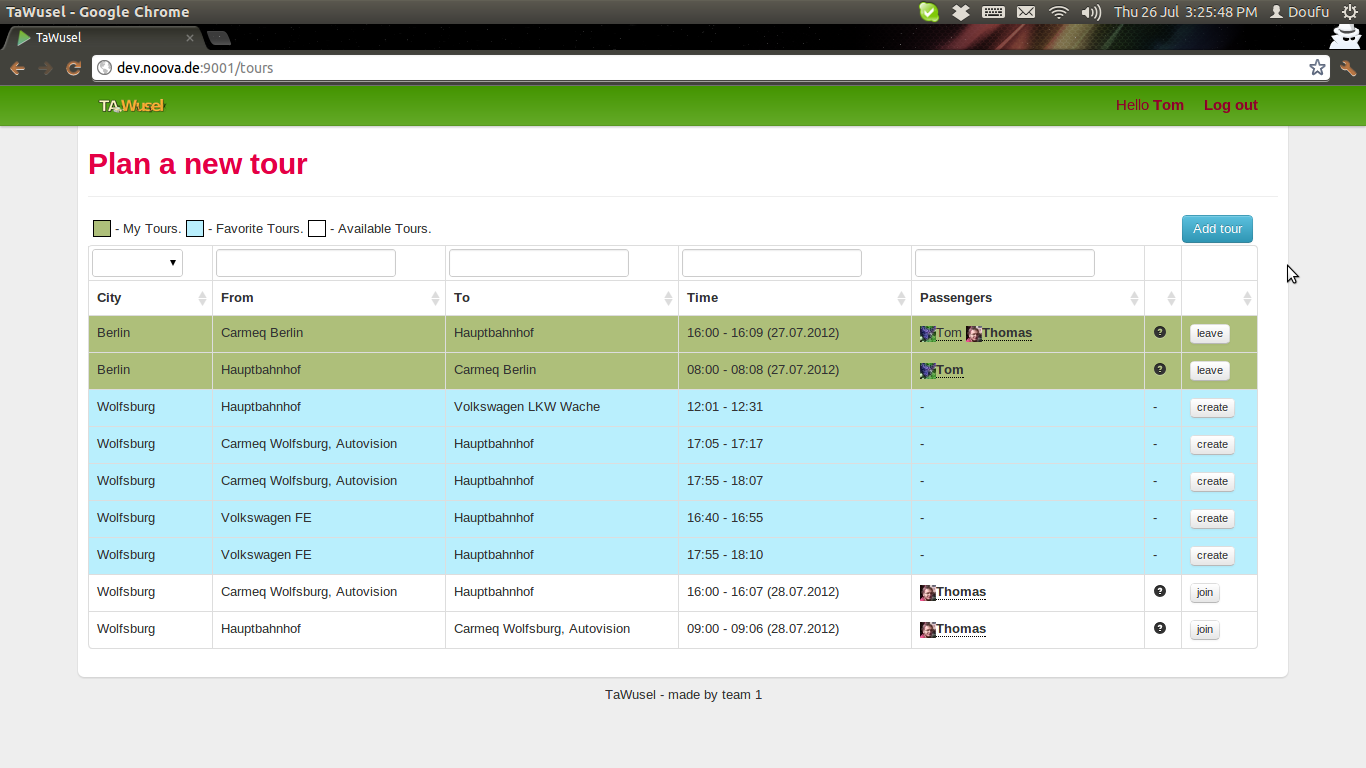
\includegraphics[width=16cm]{images/TaWusel_Web_main.png}\label{img:WebLogin}



\begin{figure}[h]
	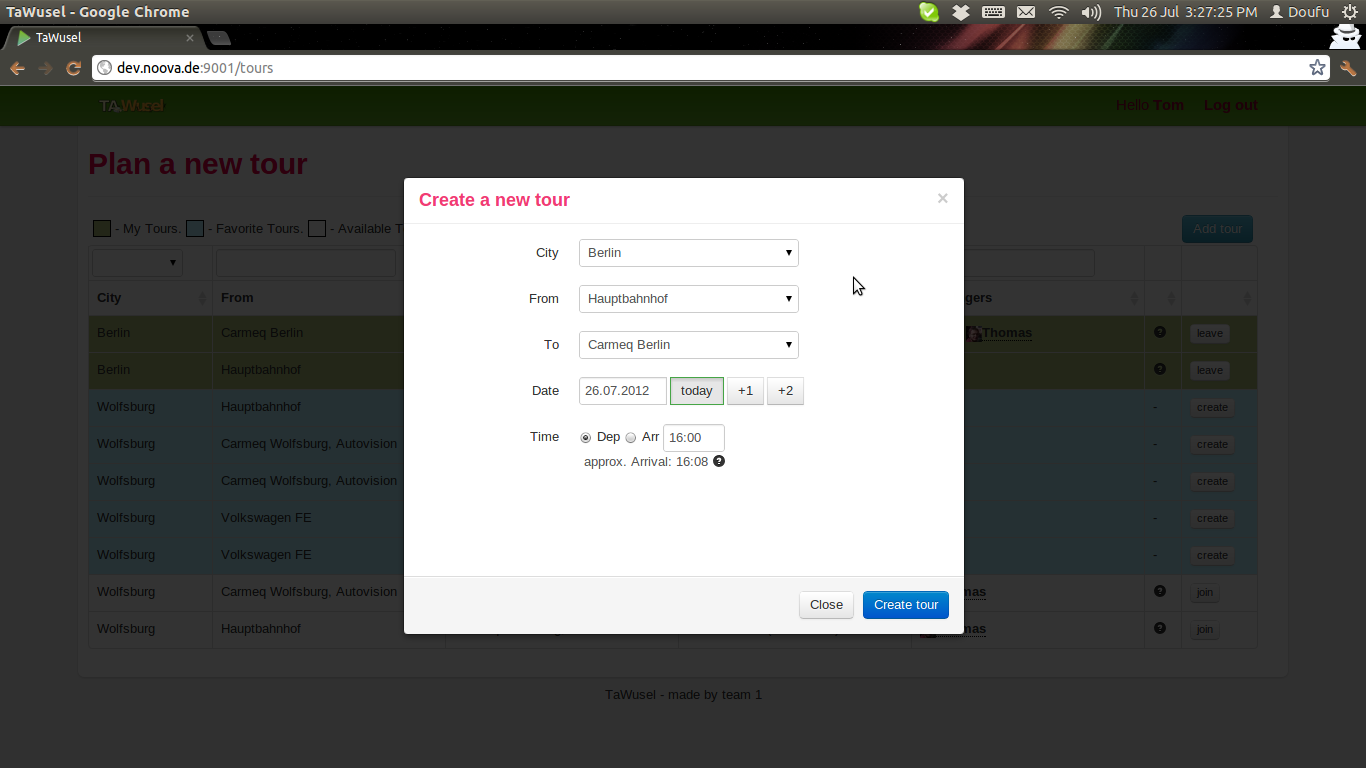
\includegraphics[width=16cm]{images/TaWusel_Web_create.png}
	\caption{modal panel for creating a tour}
	\label{img:WebLogin}
\end{figure}



\begin{figure}[h]
	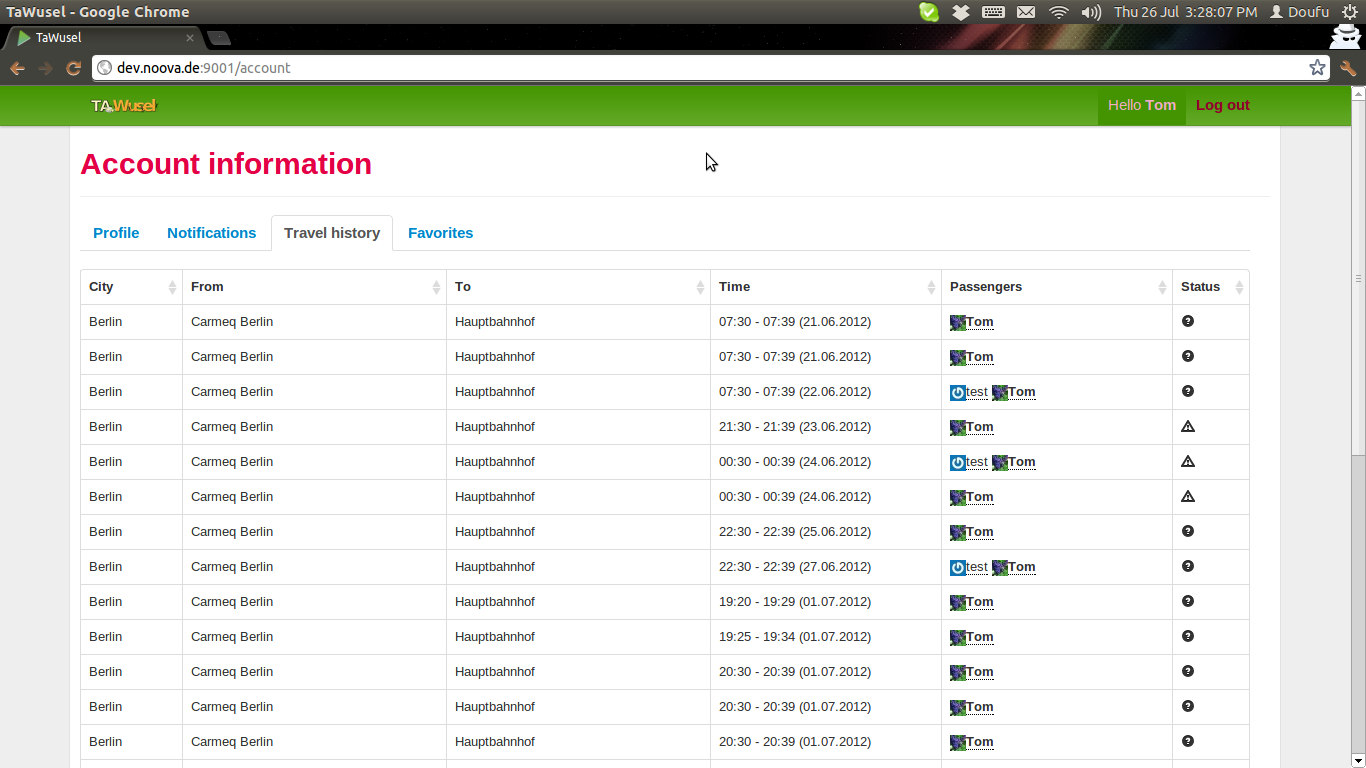
\includegraphics[width=16cm]{images/TaWusel_Web_history.png}
	\caption{profile page - history tab}
	\label{img:WebLogin}
\end{figure}
\subsection{Installation guide - Webservice}\label{ssec:WebInst}

The rough install instructions can also be found in the \texttt{INSTALL.md} file.
\begin{itemize}

\item As TaWusel uses the Play!2 framework (Scala version) obviously the first requirement is said framework. To obtain it, the
best way is to follow the official installation documentation from the Play!
website\footnote{\url{http://www.playframework.org/}}.

\item The next step is to set up a MySQL-database\footnote{In theory, other SQL-DBMS should work as well, since TaWusel uses
JDBC for its connections. However we have only used MySQL so far.} for your project.
As installing MySQL can obviously not be part of this documentation, we shall only briefly point towards the official
website\footnote{\url{http://dev.mysql.com/doc/refman/5.6/en/installing.html}} and name
XAMPP\footnote{\url{http://www.apachefriends.org/en/xampp.html}} and MAMP\footnote{\url{http://www.mamp.info}} as two easy
alternatives
for installing MySQL on Windows and Mac OS X respectively.\\
Example code for setting up the database:
\begin{verbatim}
CREATE DATABASE tawusel;
CREATE USER tawusel;
GRANT ALL ON tawusel.* TO tawusel@localhost IDENTIFIED BY 'pass';
\end{verbatim}
\small{To use other credentials, the \texttt{conf/application.conf} has to be changed accordingly.}

\item Lastly go to \url{https://github.com/nutztherookie/tawusel} and download TaWusel. Unzip, go to the project's root folder and
run \texttt{play run}.\\
Point your web browser to \url{http://localhost:9000/}


\end{itemize}